\documentclass[a4paper,10pt]{article}
\usepackage[utf8]{inputenc}
\usepackage[margin=1.5cm, bottom=2cm]{geometry}
\usepackage{fancyhdr}
\usepackage{enumitem}
\usepackage{xcolor}
\usepackage{makeidx}
\usepackage[most]{tcolorbox}
\newtcolorbox{osservazioni}{
  colback=gray!8,    % sfondo grigio chiaro
  colframe=white,      % nessun bordo
  arc=2mm,            % angoli smussati
  boxrule=0pt,        % spessore bordo 0
  fontupper=\footnotesize,
  left=2mm, right=2mm, top=2mm, bottom=2mm,
  before skip=7pt,   % niente spazio prima
  after skip=15pt     % niente spazio dopo
}
\newtcolorbox{osservazioni2}{
  colback=gray!8,    % sfondo grigio chiaro
  colframe=white,      % nessun bordo
  arc=2mm,            % angoli smussati
  boxrule=0pt,        % spessore bordo 0
  fontupper=\small,
  left=5mm, right=5mm, top=3mm, bottom=3mm,
  before skip=0pt,   % niente spazio prima
  after skip=30pt     % niente spazio dopo
}
\pagestyle{fancy}
\usepackage{tikz}
\usetikzlibrary{automata, positioning}
\pagestyle{fancy}

\usepackage{makeidx}

%%%%%%%%%%%%%%%%%%%
\newcommand{\EsercitazioneNum}{07}
\newcommand{\Data}{23/10/2025}
\newcommand{\DocType}{Esercitazione} % o "Eserciziario"
\newcommand{\FullTitle}{\DocType\ \EsercitazioneNum}

\newcommand{\Header}{
\noindent
  \small \textbf{Computabilità, Complessità e Logica - a.a. 2025/26} \hfill \textbf{\FullTitle} \\[0.2cm]
  \scriptsize Matteo Liotta, \texttt{matteo.liotta@studenti.units.it} \hfill \Data \\[0.2cm]
  \noindent\makebox[\linewidth]{\rule{\linewidth}{0.4pt}} \\[0.3cm]}

\newcommand{\NewPageHeader}{
  \vfill
  \noindent\makebox[\linewidth]{\rule{\linewidth}{0.4pt}}
  \newpage
  {\Header}
}
%%%%%%%%%%%%%%%%%%%

% Numero di pagina in basso al centro
\fancyhf{}
\fancyfoot[C] \thepage
\renewcommand{\footrulewidth}{0pt} % niente linea in basso
\renewcommand{\headrulewidth}{0pt} % niente linea in alto

\begin{document}

\footnotesize  % font generale più piccolo
\Header\\[0.7cm]


%%%%%%%%%%%%%%%% FOGLIO 2


%% INDEX
\addcontentsline{toc}{section}{Esercitazione 07: \textit{Macchine di Turing}}

\noindent\Large \textbf{Esercitazione 07}: \textit{Macchine di Turing}
\begin{osservazioni}
    \textbf{\textit{Nota}}. Sono indicati in \textcolor{blue}{\textit{blu}} gli esercizi che non saranno trattati durante l'esercitazione, bensì lasciati come strumento aggiuntivo di esercitazione individuale. Resta comunque assoluta disponibilità per la loro risoluzione negli incontri successivi, qualora necessario.
\end{osservazioni}

{\normalsize
\begin{itemize}[label=, leftmargin=0pt]

    %% INDEX
    \addcontentsline{toc}{subsection}{Esercizio 47.} 
    %%
    \item \textbf{Esercizio 47 (*)}\\ Sia $L$ linguaggio regolare su $\Sigma=\{a,b\}$, tale per cui 
    {\begin{center}
        $L = \{ w \in \Sigma^* \mid w = a^nb^n,\ \ \  n\geq0 \}$
    \end{center}} 
    Si rappresenti la macchina di Turing tale da riconoscere il linguaggio $L$.\\[0.1cm]

    \begin{osservazioni}
        \underline{\textit{Soluzione.}}\\
    Si ricorda come la parola $w$ all'inizio dell'esecuzione sia completamente inserita sul nastro. L'idea, allora, è la seguente: \textit{ad ogni lettura di una $a$ ci aspettiamo sia corrispondente la lettura di una $b$}. Questo vuol dire che, leggendo un termine $a$ sul nastro dovremo verificare la presenza di $b$. Ricordiamo come sia possibile sovrascrivere i simboli con $A$ e $B$ o altro sul nastro.\\
    
    Prima di cominciare la scrittura, consideriamo il caso con $w=a^3b^3$. In questo caso il nastro sia della forma:
    
    \begin{center}
    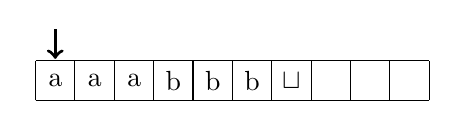
\begin{tikzpicture}[scale=0.5, every node/.style={minimum size=0.7cm}]
    
    % Nastro
    \draw (0,0) grid (10,1);
    \node at (0.5,0.5) {a};
    \node at (1.5,0.5) {a};
    \node at (2.5,0.5) {a};
    \node at (3.5,0.5) {b};
    \node at (4.5,0.5) {b};
    \node at (5.5,0.5) {b};
    \node at (6.5,0.5) {$\sqcup$};
    
    \draw[very thick,->] (0.5,1.8) -- (0.5,1.05);
    \end{tikzpicture}
    \end{center}

    Allora, ci aspettiamo che dopo la lettura di $a$, marcandola con $A$, sia possibile scorrere a destra \textit{fino all'incontro di una prima lettera } $b$:
    
    \begin{center}
    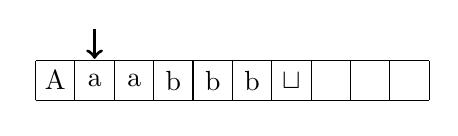
\begin{tikzpicture}[scale=0.5, every node/.style={minimum size=0.7cm}]
    
    % Nastro
    \draw (0,0) grid (10,1);
    \node at (0.5,0.5) {A};
    \node at (1.5,0.5) {a};
    \node at (2.5,0.5) {a};
    \node at (3.5,0.5) {b};
    \node at (4.5,0.5) {b};
    \node at (5.5,0.5) {b};
    \node at (6.5,0.5) {$\sqcup$};
    
    \draw[very thick,->] (1.5,1.8) -- (1.5,1.05);
    \end{tikzpicture}

    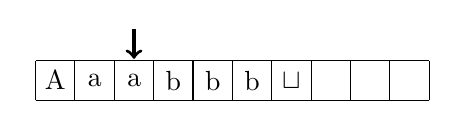
\begin{tikzpicture}[scale=0.5, every node/.style={minimum size=0.7cm}]
    
    % Nastro
    \draw (0,0) grid (10,1);
    \node at (0.5,0.5) {A};
    \node at (1.5,0.5) {a};
    \node at (2.5,0.5) {a};
    \node at (3.5,0.5) {b};
    \node at (4.5,0.5) {b};
    \node at (5.5,0.5) {b};
    \node at (6.5,0.5) {$\sqcup$};
    
    \draw[very thick,->] (2.5,1.8) -- (2.5,1.05);
    \end{tikzpicture}

    
    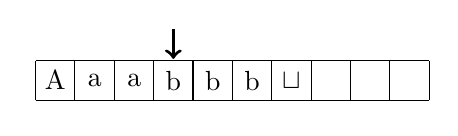
\begin{tikzpicture}[scale=0.5, every node/.style={minimum size=0.7cm}]
    
    % Nastro
    \draw (0,0) grid (10,1);
    \node at (0.5,0.5) {A};
    \node at (1.5,0.5) {a};
    \node at (2.5,0.5) {a};
    \node at (3.5,0.5) {b};
    \node at (4.5,0.5) {b};
    \node at (5.5,0.5) {b};
    \node at (6.5,0.5) {$\sqcup$};
    
    \draw[very thick,->] (3.5,1.8) -- (3.5,1.05);
    \end{tikzpicture}
    \end{center}
    Quando la testina della macchina raggiunge il primo simbolo $b$, sappiamo che è stata trovata una corrispondenza: possiamo marcarlo e tornare indietro per verificare se è presente un'altra $a$ e ricominciare il ciclo di operazioni. Idealmente, troveremo un'altra $a$, sapendo che dobbiamo scorrere indietro con la testina fino a che non incontreremo $A$ (e muoverla di conseguenza subito a destra):

    \begin{center}
    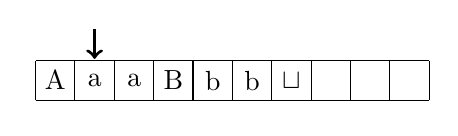
\begin{tikzpicture}[scale=0.5, every node/.style={minimum size=0.7cm}]
    
    % Nastro
    \draw (0,0) grid (10,1);
    \node at (0.5,0.5) {A};
    \node at (1.5,0.5) {a};
    \node at (2.5,0.5) {a};
    \node at (3.5,0.5) {B};
    \node at (4.5,0.5) {b};
    \node at (5.5,0.5) {b};
    \node at (6.5,0.5) {$\sqcup$};
    
    \draw[very thick,->] (1.5,1.8) -- (1.5,1.05);
    \end{tikzpicture}
    \end{center}
    
    Verrà marcata anche questa e si procederà cercando un'altra $b$, avendo cura di ignorare $B$ che si incontrerà nel percorso:

    \begin{center}
    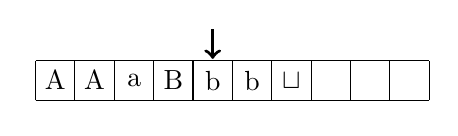
\begin{tikzpicture}[scale=0.5, every node/.style={minimum size=0.7cm}]
    
    % Nastro
    \draw (0,0) grid (10,1);
    \node at (0.5,0.5) {A};
    \node at (1.5,0.5) {A};
    \node at (2.5,0.5) {a};
    \node at (3.5,0.5) {B};
    \node at (4.5,0.5) {b};
    \node at (5.5,0.5) {b};
    \node at (6.5,0.5) {$\sqcup$};
    
    \draw[very thick,->] (4.5,1.8) -- (4.5,1.05);
    \end{tikzpicture}
    \end{center}

    Questo sarà vero per ogni coppia. Quando le $a$ saranno finite, ce ne si accorgerà dalla assenza di una $a$ a destra di $A$ e, se così, bisognerà controllare che non ci sia anche nessuna $b$ rimasta. Potremo capirlo se il prossimo simbolo dopo l'ultima $B$ sarà una $\sqcup$ (simbolo di nastro vuoto).
        \begin{center}
    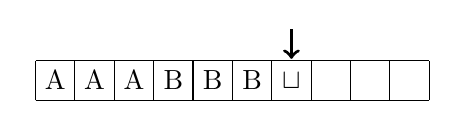
\begin{tikzpicture}[scale=0.5, every node/.style={minimum size=0.7cm}]
    
    % Nastro
    \draw (0,0) grid (10,1);
    \node at (0.5,0.5) {A};
    \node at (1.5,0.5) {A};
    \node at (2.5,0.5) {A};
    \node at (3.5,0.5) {B};
    \node at (4.5,0.5) {B};
    \node at (5.5,0.5) {B};
    \node at (6.5,0.5) {$\sqcup$};
    
    \draw[very thick,->] (6.5,1.8) -- (6.5,1.05);
    \end{tikzpicture}
    \end{center}

    \end{osservazioni}

    \NewPageHeader

    \begin{osservazioni}
    Quindi, abbiamo chiaro come sia articolato il processo alla base della macchina di Turing ad alto livello. L'interesse allora si sposta alla costruzione stessa della macchina. \\

    La macchina inizia con la lettura e la marcatura di $a$ con $A$, muovendosi a destra:

    \begin{center}
    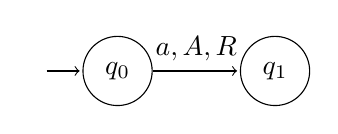
\begin{tikzpicture}[shorten >=1pt, node distance=2cm, on grid, auto]
        \node[state, initial, initial text=] (q0)   {$q_0$};
        \node[state] (q1) [right=of q0] {$q_1$};

        \path[->]
        (q0) edge  node {$a, A, R$} (q1);
    \end{tikzpicture}
    \end{center}

    Dopo la prima marcatura, ci si sposta a destra fino a che non si trova la prima $b$ sul nastro, ignorando tutto:

    \begin{center}
    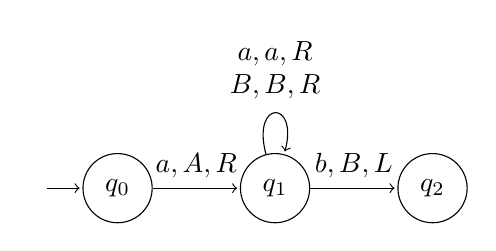
\begin{tikzpicture}[shorten >=1pt, node distance=2cm, on grid, auto]
        \node[state, initial, initial text=] (q0)   {$q_0$};
        \node[state] (q1) [right=of q0] {$q_1$};
        \node[state] (q2) [right=of q1] {$q_2$};


        \path[->]
        (q0) edge  node {$a, A, R$} (q1)
        (q1) edge [loop above] node {$\begin{array}{c} a,a,R \\ B,B,R \end{array}$} (q1)
        (q1) edge  node {$b, B, L$} (q2);

    \end{tikzpicture}
    \end{center}

    Quando viene letta una $b$ e si ritorna, si ingnora il resto per cercare un'altra $a$. Per farlo, possiamo tornare fino all'ultimo $A$, poi spostarci a destra:

    \begin{center}
    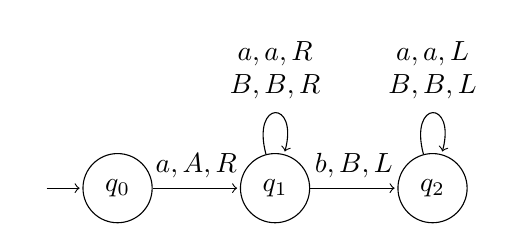
\begin{tikzpicture}[shorten >=1pt, node distance=2cm, on grid, auto]
        \node[state, initial, initial text=] (q0)   {$q_0$};
        \node[state] (q1) [right=of q0] {$q_1$};
        \node[state] (q2) [right=of q1] {$q_2$};
        %\node[state] (q3) [right=of q2] {$q_3$};
        %\node[state] (q4) [right=of q3] {$q_4$};

        \path[->]
        (q0) edge  node {$a, A, R$} (q1)
        (q1) edge [loop above] node {$\begin{array}{c} a,a,R \\ B,B,R \end{array}$} (q1)
        (q1) edge  node {$b, B, L$} (q2)
        %(q2) edge [bend right] node {$a, a, L$} (q3)
        %(q2) edge [bend left] node {$B, B, L$} (q3)
        (q2) edge [loop above] node {$\begin{array}{c} a,a,L \\ B,B,L \end{array}$} (q2);
        %(q2) edge [bend left] node {$A, A, R$} (q3)
    \end{tikzpicture}
    \end{center}

    Come visto prima, a destra di un simbolo $A$ sul nastro possiamo aspettarci la presenza di una $a$, cosa che farebbe ricominciare il ciclo portato avanti da $q1$ fino ad ora:

    \begin{center}
    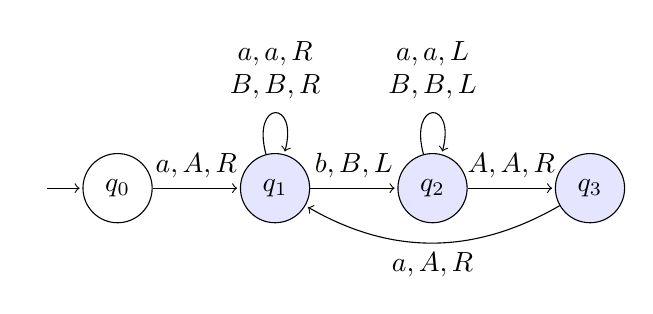
\begin{tikzpicture}[shorten >=1pt, node distance=2cm, on grid, auto]
        \node[state, initial, initial text=] (q0)   {$q_0$};
        \node[state] (q1) [right=of q0, fill=blue!10] {$q_1$};
        \node[state] (q2) [right=of q1, fill=blue!10] {$q_2$};
        %\node[state] (q3) [right=of q2, fill=blue!10] {$q_3$};
        \node[state] (q3) [right=of q2, fill=blue!10] {$q_3$};
        %\node[state] (q4) [right=of q3, fill=orange!10] {$q_4$};

        \path[->]
        (q0) edge  node {$a, A, R$} (q1)
        (q1) edge [loop above] node {$\begin{array}{c} a,a,R \\ B,B,R \end{array}$} (q1)
        (q1) edge  node {$b, B, L$} (q2)
        %(q2) edge [bend right] node {$a, a, L$} (q4)
        %(q2) edge [bend left] node {$B, B, L$} (q4)
        (q2) edge [loop above] node {$\begin{array}{c} a,a,L \\ B,B,L \end{array}$} (q2)
        (q2) edge node {$A, A, R$} (q3)
        (q3) edge [bend left] node {$a, A, R$} (q1);
        %(q3) edge node {$B, B, R$} (q4)
        %(q4) edge [loop above] node {$B, B, R$} (q4);
        
    \end{tikzpicture}
    \end{center}
    
    Eppure, potremmo anche trovare $B$, nel caso in cui fossero finite le $a$ della parola. In tal caso, dobbiamo vedere che non sia il caso di $\#a>\#b$...


    \begin{center}
    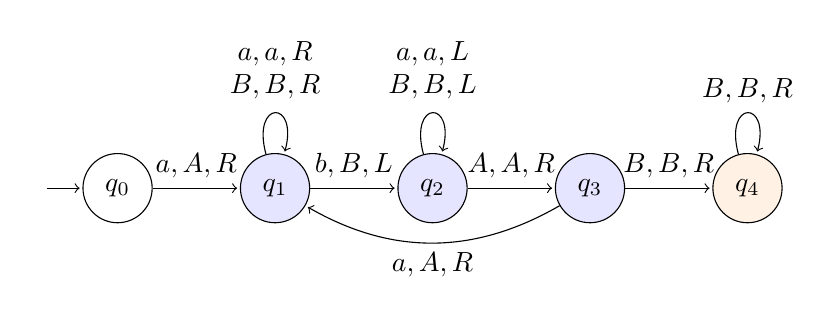
\begin{tikzpicture}[shorten >=1pt, node distance=2cm, on grid, auto]
        \node[state, initial, initial text=] (q0)   {$q_0$};
        \node[state] (q1) [right=of q0, fill=blue!10] {$q_1$};
        \node[state] (q2) [right=of q1, fill=blue!10] {$q_2$};
        %\node[state] (q3) [right=of q2, fill=blue!10] {$q_3$};
        \node[state] (q3) [right=of q2, fill=blue!10] {$q_3$};
        \node[state] (q4) [right=of q3, fill=orange!10] {$q_4$};

        \path[->]
        (q0) edge  node {$a, A, R$} (q1)
        (q1) edge [loop above] node {$\begin{array}{c} a,a,R \\ B,B,R \end{array}$} (q1)
        (q1) edge  node {$b, B, L$} (q2)
        %(q2) edge [bend right] node {$a, a, L$} (q4)
        %(q2) edge [bend left] node {$B, B, L$} (q4)
        (q2) edge [loop above] node {$\begin{array}{c} a,a,L \\ B,B,L \end{array}$} (q2)
        (q2) edge node {$A, A, R$} (q3)
        (q3) edge [bend left] node {$a, A, R$} (q1)
        (q3) edge node {$B, B, R$} (q4)
        (q4) edge [loop above] node {$B, B, R$} (q4);
        
    \end{tikzpicture}
    \end{center}
    Ci aspettiamo di terminare solo nel caso in cui, continuando ad andare a destra, incontriamo il simbolo di nastro vuoto: $\sqcup$.

    \begin{center}
    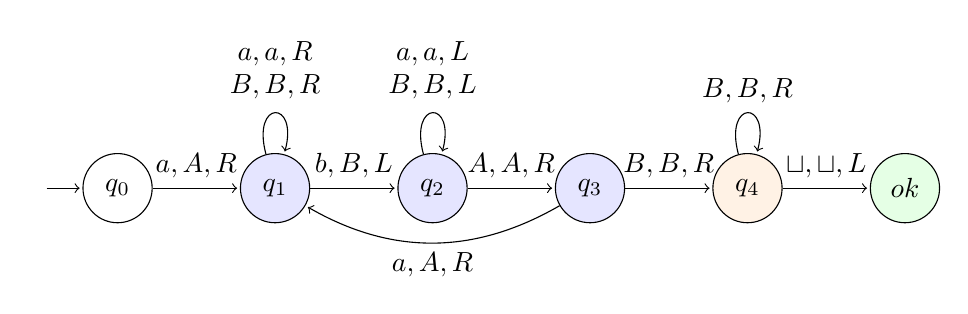
\begin{tikzpicture}[shorten >=1pt, node distance=2cm, on grid, auto]
        \node[state, initial, initial text=] (q0)   {$q_0$};
        \node[state] (q1) [right=of q0, fill=blue!10] {$q_1$};
        \node[state] (q2) [right=of q1, fill=blue!10] {$q_2$};
        %\node[state] (q3) [right=of q2, fill=blue!10] {$q_3$};
        \node[state] (q3) [right=of q2, fill=blue!10] {$q_3$};
        \node[state] (q4) [right=of q3, fill=orange!10] {$q_4$};
        \node[state] (q5) [right=of q4, fill=green!10] {$ok$};


        \path[->]
        (q0) edge  node {$a, A, R$} (q1)
        (q1) edge [loop above] node {$\begin{array}{c} a,a,R \\ B,B,R \end{array}$} (q1)
        (q1) edge  node {$b, B, L$} (q2)
        %(q2) edge [bend right] node {$a, a, L$} (q4)
        %(q2) edge [bend left] node {$B, B, L$} (q4)
        (q2) edge [loop above] node {$\begin{array}{c} a,a,L \\ B,B,L \end{array}$} (q2)
        (q2) edge node {$A, A, R$} (q3)
        (q3) edge [bend left] node {$a, A, R$} (q1)
        (q3) edge node {$B, B, R$} (q4)
        (q4) edge [loop above] node {$B, B, R$} (q4)
        (q4) edge node {$\sqcup, \sqcup, L$} (q5);

        
    \end{tikzpicture}
    \end{center}
    \end{osservazioni}
    \NewPageHeader

    
    %% INDEX
    \addcontentsline{toc}{subsection}{Esercizio 48.} 
    %%
    \item \textbf{Esercizio 48. (**)}\\ Sia $L$ linguaggio su $\Sigma=\{a,b,c\}$, tale per cui 
    {\begin{center}
        $L = \{ w \in \Sigma^* \mid w = a^{n_1}b^{n_2}c^{n_3}, n_3 = n_1+n_2, \ \ \ n_1,n_2\geq1\}$
    \end{center}} 
    Si rappresenti la macchina di Turing tale da riconoscere il linguaggio $L$.\\[0.1cm]
    
    \begin{osservazioni}
    \underline{\textit{Soluzione.}}\\
    La soluzione è simile all'esercizio precedente, solo che in questo caso dobbiamo controllare che per ogni $a$ corrisponda una $c$ e per ogni $b$ corrisponda una $c$. Possiamo sfruttare:
    \begin{itemize}
        \item L'idea della MdT del precedente esercizio;
        \item L'ordinamento che impone $a$ prima di $b$ e prima di $c$.
    \end{itemize}
    Se così, possiamo di fatto andare a gestire i due casi in maniera indipendente.
    \begin{itemize}
        \item Per ogni simbolo di $a$ letto saltiamo le $b/B$ e cerchiamo le $c$;
        \item Per ogni simbolo di $b$, ripetiamo il caso precedente (cfr. es. 47).
    \end{itemize}

    
    \begin{center}
    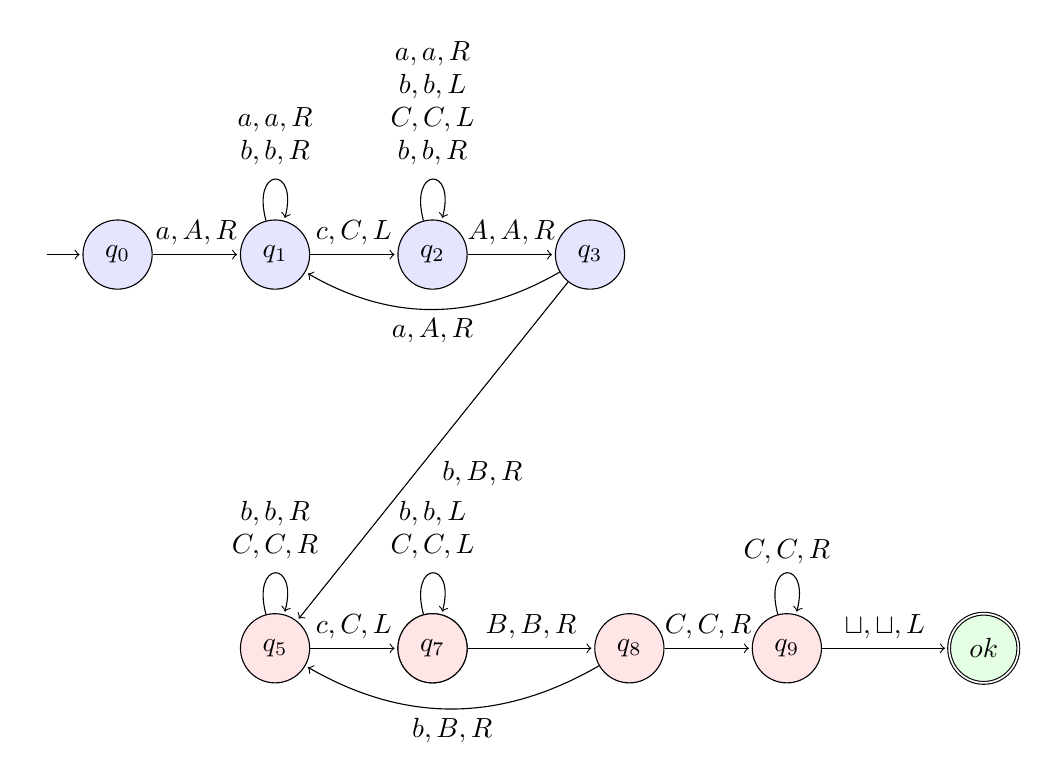
\begin{tikzpicture}[shorten >=1pt, node distance=2cm, on grid, auto]
        \node[state, initial, initial text=, fill=blue!10] (q0)   {$q_0$};
        \node[state] (q1) [right=of q0, fill=blue!10] {$q_1$};
        \node[state] (q2) [right=of q1, fill=blue!10] {$q_2$};
        \node[state] (q3) [right=of q2, fill=blue!10] {$q_3$};
        %\node[state] (q5) [right=2.5of q4, fill=blue!10] {$q_5$};

        \node[state, fill=red!10, below=5of q1] (q5)   {$q_5$};
        \node[state] (q6) [right=of q5, fill=red!10] {$q_6$};
        \node[state] (q7) [right=of q5, fill=red!10] {$q_7$};
        \node[state] (q8) [right=2.5of q7, fill=red!10] {$q_8$};
        \node[state] (q9) [right=of q8, fill=red!10] {$q_9$};
        \node[state] (q10) [accepting, right=2.5of q9, fill=green!10] {$ok$};
        %\node[state] (q6) [right=of q5, fill=blue!10] {$ok$};


        \path[->]
        (q0) edge  node {$a, A, R$} (q1)
        (q1) edge [loop above] node {$\begin{array}{c} a,a,R \\ 
                                                       %B,B,R \\ 
                                                       b,b,R \end{array}$} (q1)
        (q1) edge  node {$c, C, L$} (q2)
        %(q2) edge [bend right] node {$\begin{array}{c} a,a,R \\ 
        %                                               %B,B,L \\ 
        %                                               b,b,L \\
        %                                               C,C,L \\
        %                                               b,b,R \end{array}$} (q3)
        %(q2) edge [bend left] node {$B, B, L$} (q3)
        (q2) edge [loop above] node {$\begin{array}{c} a,a,R \\ 
                                                       %B,B,L \\ 
                                                       b,b,L \\
                                                       C,C,L \\
                                                       b,b,R \end{array}$} (q2)
        (q2) edge node {$A, A, R$} (q3)
        (q3) edge [bend left=30] node {$a, A, R$} (q1)
        (q3) edge node {$b, B, R$} (q5)
        %(q5) edge [loop above] node {$B, B, R$} (q5)
        %(q5) edge node {$\sqcup, \sqcup, L$} (q6);

                
        (q5) edge [loop above] node {$\begin{array}{c} b,b,R \\ C,C,R \end{array}$} (q5)
        (q5) edge  node {$c, C, L$} (q6)
        %(q6) edge [bend right] node {$b, b, L$} (q7)
        %(q6) edge [bend left] node {$C, C, L$} (q7)
        (q7) edge [loop above] node {$\begin{array}{c} b,b,L \\ C,C,L \end{array}$} (q7)
        (q7) edge node {$B, B, R$} (q8)
        (q8) edge [bend left=30] node {$b, B, R$} (q5)
        (q8) edge node {$C, C, R$} (q9)
        (q9) edge [loop above] node {$C, C, R$} (q9)
        (q9) edge node {$\sqcup, \sqcup, L$} (q10);

        
    \end{tikzpicture}
    \end{center}
    
    \end{osservazioni}

    %% INDEX
    \addcontentsline{toc}{subsection}{Esercizio 49.} 
    %%
    \item \textbf{Esercizio 49. (***)}\\ Si scriva una macchina di Turing $M$ che avendo una stringa $w$ in $\Sigma=\{0, 1\}^*$ termina lasciando sul nastro la stringa $w\# w'$ dove $w'$ è la rappresentazione binaria della lunghezza di $w$.\\[0.1cm]

    
    %% INDEX
    \addcontentsline{toc}{subsection}{Esercizio 50.} 
    %%
    \item \textcolor{blue}{\textbf{Esercizio 50. (*)}}\\ Sia $L$ linguaggio su $\Sigma=\{a,b,c\}$, tale per cui 
    {\begin{center}
        $L = \{ w \in \Sigma^* \mid w = a^{n_1}b^{n_2}c^{n_3}, n_3 = n_1\times n_2, \ \ \ n_1,n_2\geq 0\}$
    \end{center}} 
    Si rappresenti la macchina di Turing tale da riconoscere il linguaggio $L$.\\[0.1cm]

    
    \begin{osservazioni}
    \underline{\textit{Soluzione.}}\\
    La macchina di Turing che riconosce il linguaggio è la seguente:
    \end{osservazioni}
    \NewPageHeader

    \begin{osservazioni}

    \begin{center}
    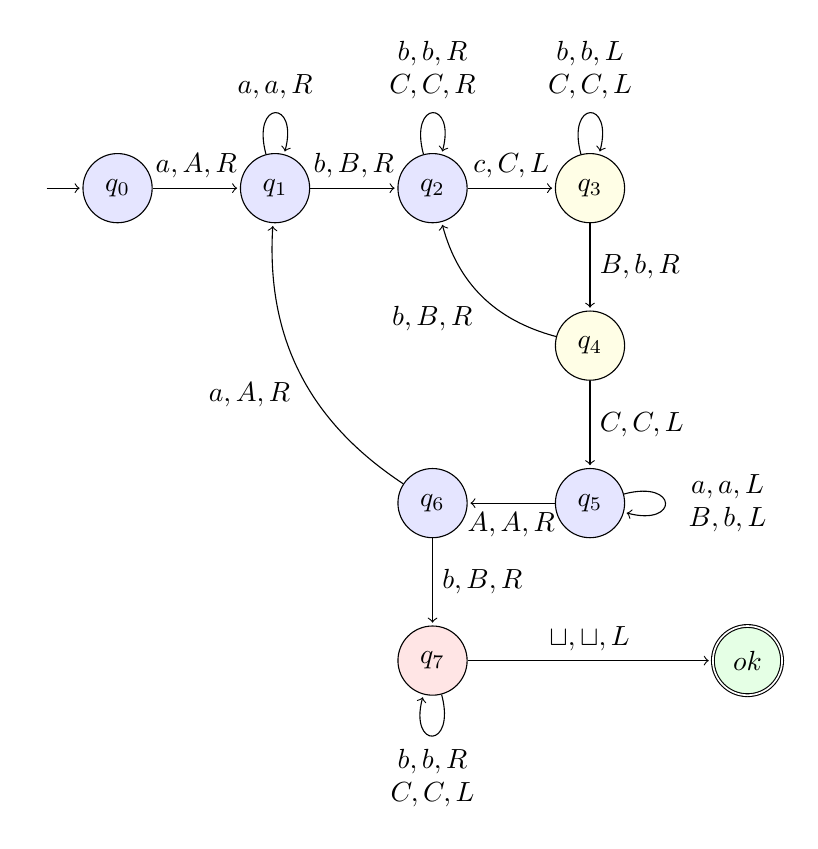
\begin{tikzpicture}[shorten >=1pt, node distance=2cm, on grid, auto]
        \node[state, initial, initial text=, fill=blue!10] (q0)   {$q_0$};
        \node[state] (q1) [right=of q0, fill=blue!10] {$q_1$};
        \node[state] (q2) [right=of q1, fill=blue!10] {$q_2$};
        \node[state] (q3) [right=of q2, fill=yellow!10] {$q_3$};
        \node[state] (q4) [below=of q3, fill=yellow!10] {$q_4$};
        \node[state] (q5) [below=of q4, fill=blue!10] {$q_5$};

        \node[state, fill=blue!10, left=of q5] (q6)   {$q_6$};
        \node[state] (q7) [below=of q6, fill=red!10] {$q_7$};
        \node[state] (q8) [accepting, right=4of q7, fill=green!10] {$ok$};
        %\node[state] (q9) [left= of q7, fill=red!15] {$X$};
        %\node[state] (q10) [right=of q9, fill=red!10] {$q_10$};
        %\node[state] (q11) [accepting, right=2.5of q10, fill=green!10] {$ok$};
        %\node[state] (q6) [right=of q5, fill=blue!10] {$ok$};

        \path[->]
        (q0) edge  node {$a, A, R$} (q1)
        (q1) edge [loop above] node {$\begin{array}{c} a,a,R\end{array}$} (q1)
        (q1) edge  node {$b, B, R$} (q2)
        (q2) edge [loop above] node {$\begin{array}{c} b,b,R\\C,C,R\end{array}$} (q2)
        (q2) edge  node {$c, C, L$} (q3)
        (q3) edge [loop above] node {$\begin{array}{c} b,b,L\\C,C,L\end{array}$} (q3)
        (q3) edge  node {$B, b, R$} (q4)
        (q4) edge  node {$C, C, L$} (q5)
        (q4) edge [bend left] node {$b, B, R$} (q2)
        (q5) edge [loop right] node {$\begin{array}{c} a,a,L\\B,b,L\end{array}$} (q5)
        (q5) edge node {$A, A, R$} (q6)
        (q6) edge [bend left] node {$a, A, R$} (q1)
        (q6) edge node {$b, B, R$} (q7)
        (q7) edge [loop below] node {$\begin{array}{c} b,b,R\\C,C,L\end{array}$} (q7)
        %(q7) edge node {$\sqcup, \sqcup, L$} (q9)
        (q7) edge node {$\sqcup, \sqcup, L$} (q8);
        
    \end{tikzpicture}
    \end{center}    
    Dove l'idea è quella di togliere una $c$ tramite riscrittura in $C$ per ogni simbolo letto $a$, un numero $b$ di volte.
    
    \end{osservazioni}
    
    
    %% INDEX
    \addcontentsline{toc}{subsection}{Esercizio 51.} 
    %%
    \item \textbf{Esercizio 51. (**)}\\ Si descriva ad alto livello una macchina di Turing $M$ che riceve in ingresso la codifica di altre due macchine di Turing (deterministiche) $M_1$ e $M_2$ e una parola $w$. Tale macchina $M$ deve accettare l'input che riceve sul nastro se la macchina  $M_1$ accetta $w$ in un numero inferiore di passi rispetto a $M_2$.

    \begin{osservazioni}
    \underline{\textit{Soluzione.}}\\
    L'esercizio non chiede la scrittura di una macchina di turing, bensì di una discussione ad alto livello. L'idea è di sfruttare una \textbf{esecuzione per passi}. Infatti:
    \begin{enumerate}
        \item $M$ accetta se $M_1$ accetta prima di $M_2$ in un numero inferiore di passi;
        \item equivalentemente, $M$ accetta se $M_1$ accetta prima di $M_2$ a parità di passi eseguiti alternandosi.
    \end{enumerate}
    Quindi, possiamo fare in modo che:
    \begin{itemize}
        \item La macchina $M$ simuli $M_1$ al passo $1$
        \item La macchina $M$ simuli $M_2$ al passo $2$
        \item La macchina $M$ torni alla situazione del passo $1$ e continui su $M_1$ al passo $3$
        \item La macchina $M$ torni alla situazione del passo $2$ e continui su $M_2$ al passo $4$
        \item ...
        \item La macchina $M$ torni alla situazione del passo $2n-1$ e continui su $M_1$ al passo $(2n-1)+2$ 
        \item La macchina $M$ torni alla situazione del passo $2n$ e continui su $M_1$ al passo $(2n)+2$ 
    \end{itemize}
    Basti allora terminare accettando appena $M_1$ accetta? Sarebbe corretto, solo avendo cura di verificare un ultimo caso che non è stato così considerato: l'eventualità di terminazione allo stesso passo per $M_1$ ed $M_2$. Poiché sappiamo che l'accettazione di $M$ è vincolata alla relazione $$\#passi_{M_1} < \#passi_{M_2}$$allora il caso di uguaglianza dovrà portare a non accettazione.
    Possiamo quindi dire che, procedendo alternando i passi:
    \begin{itemize}
        \item Se al passo $2i+1$ la macchina $M_1$ \textbf{accetta} e al passo $2i+2$ la macchina $M_2$ \textbf{non accetta} $\Rightarrow$ $M$ \textbf{accetta}
        \item Se al passo $2i+1$ la macchina $M_1$ \textbf{non accetta} e al passo $2i+1$ la macchina $M_2$ \textbf{accetta} $\Rightarrow$ $M$ \textbf{rifiuta}
        \item Se al passo $2i+1$ la macchina $M_1$ \textbf{accetta} e al passo $2i+1$ la macchina $M_2$ \textbf{accetta} $\Rightarrow$ $M$ \textbf{rifiuta}
    \end{itemize}
    
    \end{osservazioni}

    \NewPageHeader

    \begin{osservazioni}
    Allora, possiamo dire:

    \begin{verbatim}
        Struttura di M
        --------------
        MdT M con 3 Nastri
        
        Input:
         - Nastro 1: Codifica MdT M1, Codifica MdT M2, w
         - Nastro 2: _
         - Nastro 3: _

         Esecuzione:
         ----------
         1. Copio la parola w dal nastro 1 al nastro 2 e nastro 3. Il nastro 2 e 3 contengono w.
         2. Metto le testine dei nastri 2 e 3 in posizione iniziale
         3. LOOP
            3.1. Passo di computazione secondo M1 sul nastro 2
            3.2. Passo di computazione secondo M2 sul nastro 3
            
            CONTROLLO
            - Se M1 è arrivata a terminazione (accettante):
              - Se M2 non è arrivata a terminazione:
                ==> END LOOP & M accetta
              - Se M2 è arrivata a terminazione
                ==> END LOOP & M rifiuta
            - Se M1 non è arrivata a terminazione
              - Se M2 accetta:
                ==> END LOOP & M rifiuta
            - Se M1 rifiuta:
                ==> END LOOP & M rifiuta
             
    \end{verbatim}
    Si noti come le considerazioni precedenti sono di fatto collegate alle condizioni di terminazione proposte.
    \end{osservazioni}
\vfill
\noindent\makebox[\linewidth]{\rule{\linewidth}{0.1pt}}

\end{itemize}
\end{document}